\documentclass[a4paper,12pt]{report}
%\includeonly{ana_capa} %Compila apenas o(s) cap{\'\i}tulo(s) desejado
\usepackage[brazil]{babel}
\usepackage[latin1]{inputenc}
\usepackage{amsmath,amsfonts,amsthm}
\usepackage[dvips]{graphicx}
\usepackage{rotating}           % for sideways tables/figures
%\usepackage[normalem]{ulem}
\usepackage{monografia} % modifica o estilo da p{\'a}gina dos cap{\'\i}tulos
\usepackage{boxedminipage}
\usepackage{fancyheadings} % p{\~o}e a linha, t{\'\i}tulos, etc. na base e topo das p{\'a}ginas


% Define\c{c}{\~a}o das margens do texto
%
%\setlength{\voffset}{3cm}
%\setlength{\hoffset}{3cm}
\setlength{\textheight}{50pc} \setlength{\textwidth}{38pc}
\setlength{\oddsidemargin}{0.5cm} \setlength{\topmargin}{-0cm}
%\setlength{\evensidemargin}{1cm}
\setlength{\textheight}{22cm}
%\setlength{\textwidth}{17cm}

% Definindo o rodap{\'e} das p{\'a}ginas
\setlength{\footrulewidth}{0.4pt}
%
\lfoot{Valente, M.D.R}
\cfoot{}%\thepage
\rfoot{DEST/UFPA}



\begin{document}

\begin{center}
\begin{figure}
\vspace*{-2cm} \centering
\includegraphics[scale=1]{BRASAO.eps}
\vspace{\stretch{1}}
\end{figure}
\end{center}

\vspace{-1cm}

 {\centerline{\normalsize{\large \bf UNIVERSIDADE FEDERAL DO
PARÁ}}\vspace{0.3cm} \centerline{\normalsize{\large \bf INSTITUTO
CIÊNCIAS EXATAS E NATURAIS }}\vspace{0.3cm}
\centerline{\normalsize{\large \bf FACULDADE DE
ESTATÍSTICA}}\vspace{0.3cm}\centerline{\normalsize{\large }}
\vspace{4cm}

\centerline{\Large{\bf CÁLCULO DAS PROBABILIDADES I e
II}}\vspace{0.5cm} \centerline{\Large{\bf }}\vspace{5cm}


\centerline{\Large {\bf Docente: Mário Diego Rocha Valente {\it }
}}\vspace{0.5cm} \centerline{\Large {\bf  }}\vspace{0.5cm}
\centerline{\Large {\bf }} \vspace{3cm}


%\centerline{\normalsize {\bf Orientador: Prof. Joaquim Carlos
%Barbosa Queiroz,{ }{ Dr.}}} \vspace{2cm}

\centerline{\normalsize {\large \bf Belém}}
 \centerline{\normalsize {\large \bf
2009}}


\tableofcontents

\chapter{Teoria das Probabilidades}
\section{Introdução}


 A teoria dos conjuntos é a teoria matemática que trata das
propriedades dos conjuntos. Ela tem sua origem nos trabalhos do
matemático russo \textbf{Georg Ferdinand Ludwig Philipp Cantor}
(1845-1918), e se baseia na idéia de definir conjunto como uma
noção primitiva. Também chamada de teoria ingênua ou intuitiva
devido a descoberta de várias antinomias (ou paradoxos)
relacionadas a definição de conjunto. Estas antinomias na teoria
dos conjuntos conduziram a matemática a axiomatizar as teorias
matemáticas, com influências profundas sobre a lógica e os
fundamentos da matemática.



%Este Capítulo trata de algumas idéias e conceitos elementares da
%teoria dos conjuntos necessários a uma introdução moderna à teoria
%da probabilidae.

%As idéias básicas da teoria dos conjuntos foram desenvolvidas pelo
%Matemático Alemão \textbf{George Cantor} (1845-1918) em 1875
%aproximadamente.\vskip0.3cm

\begin{figure}[!htb]
\centering
  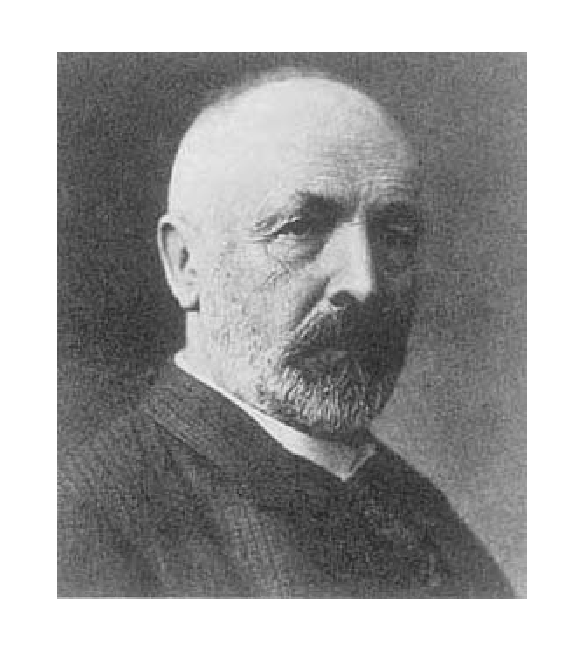
\includegraphics[scale=0.8]{cantor.eps}\\
  \vspace{-0.5cm}
  \caption{Georg Cantor.}\label{}
\end{figure}


A teoria teve seu início com a publicação em 1874 de um trabalho
de Cantor que tratava sobre a comparação de coleções infinitas. O
trabalho apresentava uma forma de comparar conjuntos infinitos
pelo "casamento" 1-1 entre os elementos destes
conjuntos.\vskip0.3cm

Desde 1638, com Galileu Galilei, sabe-se que se pode obter uma
correspondência 1-1 entre os números inteiros e seus quadrados, o
que violava a concepção euclidiana de que o todo é sempre maior
que qualquer uma de suas partes.\vskip0.3cm

Esta aplicação da correspondência 1-1 permitiu a Cantor introduzir
um método de diagonalização, que por contradição, permitia provar
que o conjunto dos números reais não tinha correspondência 1-1 com
o conjunto dos números inteiros. Isto, mais tarde, levou ao
desenvolvimento do conceito de contínuo por Richard
Dedekind.\vskip0.3cm

Iniciando com estas descobertas, Cantor acabou desenvolvendo uma
teoria dos conjuntos abstratos, que constitui-se em uma
generalização do conceito de conjunto usada até hoje em vários
ramos de pesquisa.\vskip0.3cm

\section{Conjuntos}

O conceito de conjunto é fundamental não somente no estudo da
Probabilidade e da Estatística, como para a Matemática em geral.
\emph{Qualquer lista ou coleção bem definida de entidades ou
objetos é chamada conjunto}, os objetos que individualmente formam
ou compõem a coleção ou conjunto são chamados \emph{elementos ou
membros}. Em geral, denota-se um conjunto por uma letra maiúscula
($A,B,C,...$) e um elemento do conjunto por letra minúscula
($a,b,c,...$).\vskip0.3cm

\section{Sunconjuntos}

Se todo elemento de um conjunto A é também elemento de um conjunto
B, dizemos que A é subconjunto de B, e escrevemos $A \subset B $
ou $B \supset A$ e lemos "A está contido em B", ou "B contém
A".\vskip0.3cm

Se um elemento $a$ pertence a um conjunto $C$ escrevemos $a \in
C$. Se $a$ não pertence a $C$ escrevemos $a \in C$. Se tanto $a$
como $b$ pertencem a $C$ escrevemos $a,b \in C$. A fim de que um
conjunto seja bem definido, devemos dispor de uma regra que nos
permita dizer se determinado objeto pertence ou não ao
conjunto.\vskip0.3cm

Um conjunto pode ser definido relacionando-se todos os seus
elementos, ou, quando isto não for possível, indicando uma
propriedade que seja válida para todos os elementos do conjunto, e
somente para eles.\vskip0.3cm


Existem três meneiras de descrever que objetos estão contidos no
conjunto A.

\begin{enumerate}
    \item Poderemos fazer uma lista dos elementos de A. Por
    exemplo, $A = \{ 1,2,3,4 \}$ descreve o conjunto formado pelos
    inteiros positivos 1,2,3 e 4.
    \item Poderemos descrever o conjunto A por meio de palavras.
    Por exemplo, poderemos dizer que A é formado de todos os
    números reais entre 0 e 1, inclusive.
    \item Para descrever o conjunto acima poderemos simplesmente
    escrever $A = \{ x|0\leq x \leq 1 \}$; isto é, A é o conjunto
    de todos os x, onde x é um número real entre 0 e 1, inclusive.
\end{enumerate}





%%%%%%%%%%%%%%%%%%%%%%%%%%%%%%%%%%%%%%%%%%%%%%%%%%%%%%%%%%%%%%%%%%%%%%%%%%%%%%%%%%%%%%%%%


\section{Modelos Matemáticos}

Neste capítulo examinaremos o tipo de fenômeno que estudaremos por
todo esta apostila. Além disso, formularemos um modelo matemático
que nos ajudará a investigar, de maneira bastante precisa, esse
fenômeno.\vskip0.3cm

Conforme J.Neymann, toda vez que se emprega Matemática com a
finalidade de estudar algum fenômeno deve-se começar por construir
um modelo matemático. Este modelo pode ser:
\textbf{Determinístico} ou então \textbf{Probabilístico}.


\subsection{Modelo Determinístico}
Neste modelo as condições sob as quais o experimento é execultado,
determinam o resultado do experimento. Tome-se, por exemplo, a lei
de Ohm, $V = IR$. Se R e I forem conhecidos, então V estará
precisamente determinístico.


\subsection{Modelo Não-Determinístico ou Probabilístico}
È um modelo em que de antemão não é possível explicitar ou definir
um resultado particular. Este modelo é especificado através de uma
distribuição de probabilidade. È utilizado quando se tem um grande
número de variáveis influenciando o resultado e estas variáveis
não podem ser controladas. Tome-se por exemplo, o lançamento de um
dado onde se tenta prever o número da fase que irá sair, a
retirada de uma carta de um baralho, etc.


\section{Experimentos Aleatórios}

È aquele que repetido em condições idênticas produz geralmente
resultados distintos. Por exemplo jogar uma moeda não viciada,
sabemos que a chance de sair cara é 50\%, mas não conseguimos
prever com exatidão o resultado da jogada, mesmo controlando todas
as circunstâncias relevantes ao experimento.\vskip0.3cm


\textbf{Ex1}: Lançar uma moeda três vezes. \vskip0.3cm

\textbf{Ex2}: Lançar dois dados simultaneamente. \vskip0.3cm

\subsection{Características dos Experimentos Aleatórios}

%Observando-se os experimentos acima pode-se destacar algumas
%características comuns.

\begin{itemize}
    \item Podem ser repetidos indefinidamente sob as mesmas
   condições;
   \item Não se pode adiantar um resultado particular, mas
    pode-se descrever todos os resultados possíveis;
    \item Se repetidos muitas vezes apresentarão uma regularidade
    em termos de frequências de resultados.
\end{itemize}




\section{Fenômenos Aleatórios}

O conceito de fenômeno aleatório é ligeiramente diferente do
conceito de experimento aleatório. Nos experimentos aleatórios
podemos controlar, de certa forma, fatores alheios ao problema os
quais podem influenciar os resultados do experimento, além disso,
podemos "reproduzir" o experimento com certa margem de
liberdade.\vskip0.3cm

Já nos fenômenos aleatórios nós somos meros observadores, os
fenômenos aleatórios tratados pela estatística são aqueles que
possuem "regularidade estatística", isto é, são observáveis e
suceptíveis de repetição.\vskip0.3cm

\textbf{Ex1}: Observar o número de casos de Meningite por mês em
Belém. \vskip0.3cm

\textbf{Ex2}: Observar a quantidade de chuva mensal.\vskip0.3cm




\section{Espaço Amostral ($\Omega$)}

Em um fenômeno aleatório ou probabilístico, isto é, sujeito às
leis do acaso, chamamos \emph{espaço amostral} ou \emph{espaço das
possibilidades} ao conjunto (em geral o mais detalhado possível)
de todos os resultados possíveis de ocorrer. Denota-lo-emos por
$S$ ou $\Omega$.\vskip0.3cm

Por exemplo, se jogarmos um dado vermelho e um dado preto, o
espaço amostral correspondente poderá ser descrito como segue.

$$
S_{1} =
\left[%
\begin{array}{cccccc}
  (1,1) & (2,1) & (3,1) & (4,1) & (5,1) & (6,1) \\
  (1,2) & (2,2) & (3,2) & (4,2) & (5,2) & (6,2) \\
  (1,3) & (2,3) & (3,3) & (4,3) & (5,3) & (6,3) \\
  (1,4) & (2,4) & (3,4) & (4,4) & (5,4) & (6,4) \\
  (1,5) & (2,5) & (3,5) & (4,5) & (5,5) & (6,5) \\
  (1,6) & (2,6) & (3,6) & (4,6) & (5,6) & (6,6) \\
\end{array}%
\right]
$$

onde, digamos, o primeiro número de cada par indica o ponto do
dado branco e o segundo indica o ponto do dado preto.\vskip0.3cm

Entretanto, deve-se notar que, mesmo que os dados fossem
idênticos, o espaço amostral poderia ser considerado análogo pois
a rigor, haveria também 36 resultados possíveis.


$$
S_{2} =
\left[%
\begin{array}{ccccc}
  CCCC  & CCCK  & CCKK  & CKKK  & KKKK \\
        & CCKC  & CKCK  & KCKK  &      \\
        & CKCC  & KCCK  & KKCK  &      \\
        & KCCC  & CKKC  & KKKC  &      \\
        &       & KCKC  &       &      \\
        &       & KKCC  &       &      \\
\end{array}%
\right]
$$

onde C representa cara e K coroa, em cada moeda
lançada.\vskip0.3cm

Com isso, o espaço amostral é dividido em discreto e contínuo.


\subsection{Espaço amostral discreto}

Quando as realizações do experimento denotam uma qualidade ou são
resultados de uma contagem, o espaço amostral é dito discreto,
isto é, suceptível de enumeração (finita ou infinita), nesse caso,
cada possível resultado é chamado de evento elementar $\{w_{i}\}$.
$$ \Omega = \{ (w_{1}),(w_{2}),(w_{3}),... \}  $$


\subsection{Espaço amostral contínuo}

Quando as realizações do experimento são resultados de uma
mensuração, isto é, os possíveis resultados não são enumeráveis, o
espaço amostral é chamado de contínuo. Neste caso, não faz sentido
falar em eventos elementares e, em geral, os eventos estão
constituídos por intervalos.


\section{Eventos}

Qualquer subconjunto de um espaço amostral será um evento,
definindo um resultado bem determinado. Os eventos podem ser
simples ou compostos, conforme se constituam de um ou mais
resultados de $S$. Designaremos os eventos por letras maiúsculas.


\subsection{Operações com Eventos}

Sejam A e B dois eventos associados a um espaço amostral.

\begin{enumerate}
    \item Se A e B forem eventos, a união entre A e B, denotada por, $A \cup B$ será o evento que
    ocorrerá se, e somente se, A ou B (ou ambos) ocorrerem.
    \item Se A e B forem eventos, a interseção entre A e B, denotada por, $A \cap B$ será o evento que
    ocorrerá se, e somente se, A e B ocorrerem.
    \item Se A for um evento, $\bar{A}$ será o evento complementar que ocorrerá
    se, e somente se, \emph{não ocorrer A}.
    \item Se A e B forem eventos, a diferença de A e B, denotada
    por $A-B$, será o evento que aqueles elementos que estão em A mas
    não estão em B ocorrerá.
    \item Dois eventos, A e B, são \emph{mutuamente excludentes}, se eles
    não puderem ocorrer juntos. Exprimiremos isso escrevendo $A \cap B =
    \phi$, isto é, a interseção de A e B é o \emph{conjunto vazio}.
\end{enumerate}


\begin{figure}[!htb]
\centering
  % Requires \usepackage{graphicx}
  \includegraphics[scale=1]{fig6.eps}\\
  \vspace{-1cm}
  \caption{Principais Operações com Eventos.}\label{}
\end{figure}

%%%%%%%%%%%%%%%%%%%%%%%%%%%%%%%%%%%%%%%%%%%%%%%%%%%%%%%%%%%%%%%%%%%%%%%%%%%%%%%%%%%%%%%%%%%%
\newpage

\subsection{Propriedades das Operações}

\begin{enumerate}
    \item Comutativa
$$A \cup B = B \cup A$$
$$A \cap B = B \cup A$$
    \item Associativa
$$A \cup (B \cup C) = (A \cup B)\cup C$$
$$A \cap (B \cap C) = (A \cap B)\cap C$$
    \item Distributiva
$$A \cup (B \cap C) = (A \cup B)\cap (A \cup C)$$
$$A \cap (B \cup C) = (A \cap B)\cup (A \cap C)$$
    \item Leis de Morgan
$$ (A \cup B)^{c}= A^{c} \cap B^{c}$$
$$ (A \cap B)^{c}= A^{c} \cup B^{c}$$
\item Geral
$$ A \cup \phi = A$$
$$ A \cap \phi = \phi$$
$$ \bar{\bar{A}}=A $$
$$ A \cup \bar{A}= \Omega $$
\end{enumerate}




%\newpage

\section{Conceitos de Probabilidade}

Historicamente, a probabilidade foi objeto de ampla discussão,
tendo sido definida de maneiras diferentes. Assim, houve a
definição de probabilidade como sendo o limite da frequência
relativa de ocorrência de um evento quando o número de provas
tendia ao infinito. Esta definição, dita \textbf{frequêntista},
padecia evidentimente de uma grande limitação.\vskip0.3cm



Uma segunda definição, conhecida por \textbf{clássica}, concebia a
probabilidade como sendo quociente do número de casos favoráveis
ao evento pelo número de casos possíveis, desde que todos
igualmente prováveis. Esta definição é hoje considerada uma regra
prática para a atribuição das probabilidades, quando
aplicável.\vskip0.3cm

Há também a se considerar as probabilidades subjetivas, atribuídas
conforme a avaliação de cada um e em geral usadas quando não há
formas objetivas de atribuição que possam se usadas.\vskip0.3cm

Modernamente, se adota a definição \textbf{axiomática} da
probilidade, proposta em 1933 pelo probabilista russo
\textbf{Kolmogorov}, segundo a qual a probabilidade obdece a três
axiomas.\vskip0.3cm





\subsection{Definição Frequentista de Probabilidade}

Na prática acontece que nem sempre é possível determinar a
probabilidade de um evento. Neste caso é necessário ter um método
de aproximação desta probabilidade. Um dos métodos utilizados é a
exeperimentação que objetiva estimar o valor da probabilidade de
um evento A com base em valore reais. A probabilidade avaliada
através deste processo é denominada de probabiliade
empírica.\vskip0.3cm


Seja $\varepsilon$ um experimento e A um evento de um espaço
amostral associado ao experimento E. Suponha-se que E seja
repetido n vezes e seja m o número de vezes que A ocorre nas n
repetições de E. Então a frequência relativa do evento A, anotada
por $fr_{a}$, é o quociente:

\begin{equation}\label{}
 fr_{a}=\frac{m}{n}
\end{equation}


\subsection{Propriedades da Frequência Relativa}

Seja $\varepsilon$ um experimento e A e B dois eventos de um
espaço amostral associado S. Sejam $f_{r_{A}}$ e $f_{r_{B}}$ e as
frequências relativas de A e B respectivamente.
Então\begin{enumerate}
    \item[{i})] $0 \leq f_{r_{A}} \leq 1$, isto é, a frequência
    relativa do evento A é um número que varia entre 0 e 1.
    \item[{ii})] $f_{r_{A}}=1$ se e somente se, A ocorre em todas
    as n repetições de $\varepsilon$.
    \item[{iii})] $f_{r_{A}}=0$ se e somente se, A nunca ocorre nas n repetições de $\varepsilon$.
    \item[{iv})] $f_{r_{A \cup B}}= f_{r_{A}}+f_{r_{B}}$ se A e B
    forem eventos mutuamente excludentes.
\end{enumerate}




\subsection{Definição Clássica de Probabilidade}

Seja E um experimento aleatório e S um espaço amostral associado
formado por $n$ resultados igualmente prováveis. Seja $A \subseteq
S$ um evento com m elementos.  A probabilidade de A, anotada por
P(A), lê-se p de A, é definida como sendo:

\begin{equation}\label{}
    P(A)= \frac{m}{n}
\end{equation}

Isto é, a probabildade do evento A é o quociente entre o número m
de casos favoráveis e o número n de casos possíveis.\vskip0.3cm


\textbf{Exemplo:} Calcular a probabilidade de no lançamento de um
dado equilibrado obter-se:

\begin{enumerate}
    \item Um resultado igual a 4.
    \item Um resultado ímpar.
\end{enumerate}

$$
P(A)= \frac{m}{n}=\frac{1}{6}=16,67\%
$$

$$
P(B)= \frac{m}{n}=\frac{3}{6}=50\%
$$


\subsection{Crítica à Definição Clássica}
A definição clássica é dúbia, já que a idéia de igualmente
provável é a mesma de com probabilidade igual, isto é, a definição
é circular, porque está definindo essencialmente a probabilidade
com seus próprios termos. A definição não pode ser aplicada quando
o espaço amostral é infinito.

\subsection{Definição Axiomática de Probabilidade}

\subsection{O que é Axiomática ?}

Em determinado ponto da evolução de uma teoria de pensamento
matemático, torna-se imperioso ordenar, sistematizar e relacionar
todos os conhecimentos entretanto nela reconhecidos, isto é,
proceder à sua \textbf{Axiomatização}.

\begin{itemize}
    \item axiomatizar consiste em escolher algumas afirmações que podem ser
feitas sobre os objectos matemáticos em estudo, na área
considerada.
    \item Delas, por processo dedutivo, obter todas as demais proposições que constituem o corpo de conhecimento da teoria em causa.
\end{itemize}

Essas afirmações, das quais deduzimos todas as outras, são os
\textbf{Axiomas} e o seu conjunto constitui uma
\textbf{Axiomática}.\vskip0.3cm

Os axiomas, além de se basearem numa aceitação por evidência,
devem ser :

\begin{itemize}
    \item logicamente independentes isto é, nenhum deles deve ser passível de se obter dos restantes;
    \item compatíveis, isto é, os axiomas não podem, por dedução lógica, conduzir a proposições contraditórias.
\end{itemize}

Às afirmações que se obtêm dedutivamente a partir dos axiomas, ou
de outras já deles obtidas por dedução, chamamos
\textbf{Teoremas}.\vskip0.3cm



Em 1933, Kolmogorov estabeleceu a definição de probabilidade por
\textbf{Axiomatização}, na sua obra \textbf{Foundations of the
Theory of Probability}. Foi com base nas propriedades das
frequências relativas e das operações sobre conjuntos que
Kolmogorov concebeu a primeira construção Axiomática Geral para a
Teoria das Probabilidades.\vskip0.3cm


Seja E um experimento aleatório com um espaço amostral associado.
A cada evento $A \subseteq S$ associa-se um número real,
representado por $P(A)$ e denominado de probabilidade de A, que
satisfaz as seguintes propriedades(axiomas).

\begin{enumerate}
    \item $0 \leq P(A) \leq 1$, a probabilidade de qualquer acontecimento A é um número real não
negativo.
    \item $P(S)=1$, a probabilidade do acontecimento certo é 1.

     \item Se A e B são eventos mutuamente excludentes, $P(A \cup
     B)=P(A)+P(B)$, se A e B são acontecimentos incompatíveis, a probabilidade de «A
ou B» é a soma das probabilidades de A e de B.

     \item Se $A_{1},A_{2},...,A_{n},...$ forem, dois a dois,
     eventos mutuamente excludentes, então,
     $P(\bigcup_{i=1}^{\infty})=P(A_{1})+P(A_{2})+...+P(A_{n})+...
     = \sum_{i=1}^{n}P(A_{i})$
\end{enumerate}

\subsection{Consequências dos Axiomas(Propriedades)}

\begin{enumerate}
    \item Se $\phi$ for o conjunto vazio, então
    $P(\phi)=0$.

\textbf{Demostração}: Para qualquer evento $A$, podemos escrever
$A=A\cup \phi$. Uma vez que $A$ e $\phi$ são mutuamente
excludentes, decorre que, $P(A)=P(A\cup \phi)= P(A)+P(\phi)$,
assim, $P(A)- P(A)= P(\phi)= 0$.
    \item Se $\bar{A}$ for o evento complementar de $A$, então
    $P(A)=1-P(\bar{A})$.

\textbf{Demostração}: Podemos escrever $\Omega = A \cup \bar{A}$
e, então, $P(\Omega)= P(A)+ P(\bar{A})$, assim, a $P(\Omega)=1$,
com isso, $1= P(A)+P(\bar{A})$, ou seja, $P(\bar{A})= 1- P(A)$.
    \item Se A e B forem dois eventos \emph{quaisquer}, então $P(A\cup B)=P(A)+P(B)-P(A\cap B)$

\textbf{Demostração}: A idéia desta demostração é decompor $A\cup
B$ e $B$ em dois eventos mutuamente excludentes e, em seguida,
aplicar a propriedade da soma. Desse modo escreveremos,

$$A \cup B= A\cup (B\cap \bar{A})$$
$$B= (A \cap B) \cup (B\cap \bar{A})$$

consequentemente,

$$P(A \cup B)= P(A)+P(B \cap \bar{A})$$
$$ P(B) = P(A \cap B) + P(B \cap \bar{A})$$

Subtraindo a segunda igualdade da primeira, obtém-se

$$ P(A \cup B) - P(B) = P(A)- P(A \cap B)$$
 e daí chega-se ao resultado

$$ P(A \cup B) = P(A)+P(B)- P(A \cap B)$$
    \item Se A, B e C forem três eventos quaisquer, então $P(A \cup B \cup C) = P(A)+P(B)+P(C)-P(A\cap B)-P(A\cap C)-P(B\cap C)+P(A\cap B \cap C)$


\textbf{ \maltese Demostração}: A demostração consiste em escrever
$A \cup B \cup C$ na forma $(A \cup B)\cup C$ e aplicar o
resultado do teorema anterior. Deixa-se a cargo do estudante
completar a demostração.

    \item Se $A \subset B$, então $P(A) < P(B)$
\end{enumerate}

\textbf{Demostração}: Podemos decompor B em dois eventos
mutuamente excludentes, na seguinte forma $B = A \cup (B \cap
\bar{A})$. Consequentemente, $P(B) = P(A)+ P(B \cup \bar{A}) \geq
P(A)$, porque $P(B \cap \bar{A}) \geq 0$.


\section{Probabilidade Condicionada}

Seja A e B dois eventos associados ao experimento $\varepsilon$.
Denotaremos por P(B/A) a probabilidade condicionada do evento B,
Quando A tiver ocorrido.\vskip0.3cm

Sempre que calcularmos P(B/A), estaremos essencialmente calculando
P(B) em relação ao espaço amostral reduzido A, em lugar de fazê-lo
em relação ao espaço amostral original $S$.\vskip0.3cm

Quando calcularmos P(B) estaremos nos perguntando quão provável
será estarmos em B, sabendo que devemos estar em S. È quando
calcularmos P(B/A) estaremos perguntando quão provável será
estarmos em B, sabendo que devemos estar em A. Isto é, o espaço
amostral ficou reduzido de S para A.


%\begin{center}
%\fbox{$\displaystyle x=\frac{-b\pm\sqrt{b^2-4ac}}{2a}$}
%\end{center}

\begin{equation}\label{}
    P(B/A) = \frac{P(A \cap B)}{P(A)}, \quad \quad desde \quad que
    \quad P(A)>0.
\end{equation}

\begin{equation}\label{}
    P(A/B) = \frac{P(A \cap B)}{P(B)}, \quad \quad desde \quad que
    \quad P(B)>0.
\end{equation}

È simples verificar as seguintes propriedades de P(B/A) para A
fixado:

\begin{enumerate}
    \item $0 \leq P(B/A) \leq 1$
    \item $P(S/A)=1$
     \item $P(B_{1} \cup B_{2}/A) = P(B_{1}/A)+P(B_{2}/A)$ se os
     eventos $B_{1}$ e $B_{2}$ forem mutuamente execludentes, $B_{1}\cap B_{2}=\emptyset$
     \item $P(B_{1} \cup B_{2} \cup ... / A) =
     P(B_{1}/A)+P(B_{2}/A)+...$ se $B_{i}\cup B_{j}=\phi$ para $i\neq
     j$.
\end{enumerate}



\textbf{Exemplo 1}: Dois Dados equilibrados são lançados,
registrando-se o resultado como ($x_{1},x_{2}$), onde $x_{i}$ é o
resultado do i-ésimo dado, i=1,2. Por isso, o espaço amostral S
pode ser representado pela seguinte lista de 36 resultados
igualmente prováveis.


$$
\Omega =
\left[%
\begin{array}{cccccc}
  (1,1) & (2,1) & (3,1) & (4,1) & (5,1) & (6,1) \\
  (1,2) & (2,2) & (3,2) & (4,2) & (5,2) & (6,2) \\
  (1,3) & (2,3) & (3,3) & (4,3) & (5,3) & (6,3) \\
  (1,4) & (2,4) & (3,4) & (4,4) & (5,4) & (6,4) \\
  (1,5) & (2,5) & (3,5) & (4,5) & (5,5) & (6,5) \\
  (1,6) & (2,6) & (3,6) & (4,6) & (5,6) & (6,6) \\
\end{array}%
\right]
$$

Considere os dois eventos seguintes:\vskip0.3cm

$A=\{(x_{1},x_{2}|x_{1}+x_{2}=10)\}$

$B=\{(x_{1},x_{2}|x_{1}>x_{2})\}$

\vskip0.3cm

Calcular:

\begin{enumerate}
    \item P(B/A)
    \item P(A/B)
\end{enumerate}


$$P(B/A)=\frac{P(A \cap
B)}{P(A)}=\frac{\frac{1}{36}}{\frac{3}{36}} = \frac{1}{3}$$


$$P(A/B)=\frac{P(A \cap
B)}{P(B)}=\frac{\frac{1}{36}}{\frac{15}{36}} = \frac{1}{15}$$

O evento $A \cap B$ ocorre se, e somente se, a soma dos dois dados
for 10 e se o primeiro dado tiver apresentado um valor maior que o
segundo dado.\vskip0.3cm


\textbf{Exemplo 2}: Uma caixa comtém duas moedas. Uma honesta e
outra com 2 caras. Uma moeda é escolhida aleatoriamente,
arremessada e o resultado observado é cara. Qual a probabilidade
de que o outro lado desta moeda escolhida, seja cara?\vskip0.3cm

Considere os seguintes Eventos.\vskip0.3cm

B=\{o resultado é cara\}.

A=\{A moeda é a de 2 caras\}

\vskip0.3cm

Calcular:

\begin{enumerate}
    \item P(A/B)
    \item P(B/A)
\end{enumerate}


$$P(A/B)=\frac{P(A \cap
B)}{P(B)}=\frac{\frac{2}{4}}{\frac{3}{4}} = \frac{2}{3}$$

Das 4 faces que podem ocorrer, 3 são caras, e duas são caras, com
caras no outro lado da moeda de 2 caras.\vskip0.3cm


A maior consequência da definição de probabilidade condicionada
acima, é obtida ao se escrever:


$$
P(A \cap B)= P(B/A)P(A)
$$
 ou equivalentemente,

$$
P(A \cap B)= P(A/B)P(B)
$$

Isto é, algumas vezes mencionado como o \textbf{Teorema da
Multiplicação} de probabilidade. Podemos aplicar esse teorema para
calcular a probabilidade da ocorrência conjunta dos eventos A e B.
\vskip0.3cm

O teorema da multiplicação de probabilidades pode ser generalizado
para mais de dois eventos, da seguinte maneira:

\begin{equation}\label{}
    P[A_{1} \cap A_{2} \cap ... \cap A_{n}]=
    P(A_{1})P(A_{2}/A_{1})P(A_{3}/A_{1},A_{2})...P(A_{n}/A_{1},...A_{n-1})
\end{equation}

Até aqui empregamos o conceito de probabilidade condicionada a fim
de avaliar a probabilidade de ocorrência conjunta de dois eventos.
Poderemos aplicar esse conceito em outra maneira de calcular a
probabilidade de um evento simples A. Necessitaremos da seguinte
definição:\vskip0.3cm


Dizemos que os eventos $B_{1},B_{2},...,B_{k}$ representam uma
\textbf{Partição do Espaço Amostral S}, quando


\begin{enumerate}
    \item $B_{i} \cap B_{j}=\phi$, para todo $i\neq j$
    \item $\bigcup^{k}_{i=1}=S$
    \item $P(B_{i})>0$ para todo $i$
\end{enumerate}

Explicando: Quando o experimento $\varepsilon$ pe realizado
\textbf{um}, \textbf{e somente um}, dos eventos $B_{i}$
ocorre.\vskip0.3cm

\textbf{Exemplo 1}: Na jogada de um dado,
$B_{1}=\{1,2\},B_{2}=\{3,4,5 \}$ e $B_{3}=\{6\}$ representariam
uma partição do espaço amostral, enquanto $C_{1}=\{1,2,3,4\}$ e
$C_{2}=\{4,5,6 \}$ não o representariam.\vskip0.3cm

Consideremos A um evento qualquer referente a S, e
$B_{1},B_{2},...,B_{k}$ uma partição de S. Poderemos escrever

$$
A = (A \cap B_{1}) \cup (A \cap B_{2}) \cup ... \cup (A \cap
B_{k}).
$$

Naturalmente, alguns dos conjuntos $A \cap B_{j}$ poderão ser
vazios, mas isso não invalida essa decomposição de A. O ponto
importante é que todos os eventos $A \cap B_{1},...,A \cap B_{k}$
são dois a dois mutuamente excludentes. Por isso, poderemos
aplicar a propriedade da adiçãos de eventos mutuamente
excludentes, e escrever


$$
P(A)=P(A\cap B_{1})+P(A\cap B_{2})+...+P(A\cap B_{k})
$$

Contudo, cada termo $P(A\cap B_{j})$ pode ser expresso na forma
$P(A/B_{j})P(B_{j})$ e, daí, obteremos o que se denomina o
\textbf{Teorema da Probabilidade Total}:

\begin{equation}\label{}
P(A)=P(A/B_{1})P(B_{1})+P(A/B_{2})P(B_{2})+...+P(A/B_{k})P(B_{k})
\end{equation}

Este resultado representa uma relação extremamente útil, porque
frequentemente, quando P(A) é pedida, pode ser difícil calculá-la
diretamente. No entanto, com a informação adicional de que $B_{j}$
tenha ocorrido, seremos capazes de calcular $P(A/B_{j})$ e, em
seguida, empregar a fórmula acima.









\section{Teorema de Bayes}
\subsection{Quem foi Thomas Bayes}

Sir \emph{Thomas Bayes} foi um matemático britânico e um ministro
da igreja presbiteriana que primeiro utilizou a probabilidade
indutivamente e estabeleceu as bases matemáticas para a inferência
probabilística. Ele nasceu em Londres, em 1702, morreu em
Tunbridge Wells em 1761 (tendo vivido apenas 59 anos), e foi
sepultado no cemitério Bunhill Fields em Londres, onde sua tumba
pode ser facilmente encontrada com o mapa fornecido pelo
cemitério.\vskip0.3cm

Seu trabalho com as probabilidades foi reunido em um ensaio
publicado após a sua morte (em 1763) no livro Philosophical
Transactions of the Royal Society of London. O ensaio Essay
Towards Solving a Problem in the Doctrine of Chances relatou,
entre outras importantes descobertas de Bayes, o famoso Teorema de
Bayes.

\subsection{ O Que É o Teorema de Bayes}

O teorema de Bayes é usado na inferência estatística para
atualizar estimativas da probabilidade de que diferentes hipóteses
sejam verdadeiras, baseado nas observações e no conhecimento de
como essas observações se relacionam com as hipóteses.\vskip0.3cm

Este teorema é uma das pedras angulares da estatística das
probabilidades combinadas, e é largamente utilizada em áreas a
primeira vista pouco relacionadas, como Medicina e
Informática.\vskip0.3cm

Na primeira, o paradigma embasado em evidências é todo construído
em cima do teorema de Bayes. Baseado na experiência acumulada de
exames e testes para tentar diagnosticar uma doença, o médico
enquadra seus pacientes e pode estimar qual a probabilidade de que
uma dada doença esteja se manifestando. Ou seja, dada uma
probabilidade inicial (por exemplo, o paciente é fumante) e
aplicado um exame em que, se sabe, há uma probabilidade de
falsos-positivos e falso-negativos (por exemplo, uma biópsia de
pulmão), o médico sabe qual a probabilidade resultante daquele
paciente ter a doença (por exemplo, câncer de pulmão).\vskip0.3cm

Na informática, muitos dos sistemas de classificação automática
são baseados no teorema de Bayes. Inicialmente o sistema é
treinado, aceitando entradas de humanos que dizem que uma dada
entrada pertencem a determinado grupo. Com o tempo, o sistema
acumula um grande banco dessas informações e, aplicando o teorema
de Bayes, consegue estimar a probabilidade de cada novo dado de
pertencer a cada grupo já classificado.\vskip0.3cm


\subsection{Definição}

Seja $B_{1},B_{2},...,B_{k}$ uma partição do espaço amostral S e
seja A um evento associado a S. aplicando-se a definição de
probabilidade condicionada, poderemos escrever


\begin{equation}\label{bayes}
    P(B_{i}/A)=\frac{P(A/B_{i})P(B_{i})}{\sum_{j=1}^{k}P(A/B_{j})P(B_{j})}
\end{equation}


Esse resultado é conhecido como \emph{Teorema de Bayes}. È também
denominado fórmula da probabilidade das causas (ou dos
antededentes). Desde que os $B_{i}$ constituam uma partição do
espaço amostral um, e somente um, dos eventos $B_{i}$ ocorrerá.


\section{Eventos Independentes}

Já consideramos eventos A e B que não podem ocorrer conjuntamente,
isto é, $A\cap B = \phi$. Tais eventos são denominados mutuamente
excludentes, ou eventos incompatíveis. Observamos anteriormente
que se A e B forem mutuamente excludentes, então $PA/B=0$, porque
a ocorrência dada de B impede a ocorrência de A. No outro extremo,
temos a situação já estudada, na qual $B \supset A$ e,
consequentemente, $P(B/A)=1$.\vskip0.3cm

Consideremos $P(A \cap B)$, supondo que as probabilidades
condicionadas sejam iguais às correspondentes probabilidades
absolutas. Teremos:

$$
P(A \cap B)= P(A/B)P(B)=P(A)P(B)
$$

$$
P(A \cap B)= P(B/A)P(A)=P(B)P(A)
$$


Desse modo, desde que nem P(A) nem P(B) sejam iguais a zero,
verificamos que as probabilidades absolutas serão iguais às
probabilidades condicionais se, e somente se, $P(A \cap
B)=P(A)P(B)$. Em consequência, formulamos a seguinte definição, a
qual será também válida quer P(A) ou P(B) seja nulo:\vskip0.3cm

\textbf{Definição:} A e B serão eventos independentes se, e
somente se,

$$
P(A \cap B) = P(A)P(B)
$$


Será importante para nós, estendermos a noção de independência
para mais de dois eventos. Consideremos, inicialmente, três
eventos associados a um experimento, digamos A, B e C. Se A e B, A
e C, B e C forem independentes dois a dois (no sentido acima),
então não se concluirá, em geral, que não exista dependência entre
os três eventos.\vskip0.3cm

\textbf{Definição:} Diremos que os três eventos A, B e C são
mutuamente independentes se, e somente se, todas as condições
seguintes forem válidas:

$$
P(A \cap B)=P(A)P(B)
$$

$$
P(A \cap C)=P(A)P(C)
$$

$$
P(B \cap C)=P(B)P(C)
$$

$$
P(A \cap B \cap C)=P(A)P(B)P(C)
$$


Finalmente, generalizando esta noção para n eventos, na seguinte
definição:\vskip0.3cm



\textbf{Definição:} Os n eventos $A_{1},A_{2},...,A_{n}$ serão
mutuamente independentes se, e somente se, tivermos para
$k=2,3,...,n$:

\begin{equation}\label{}
    P(A_{i_{1}} \cap A_{i_{2}} \cap A_{i_{k}})=
    P(A_{i_{1}})P(A_{i_{2}})...P(A_{i_{k}})
\end{equation}




%%%%%%%%%%%%%%%%%%%%%%%%%%%%%%%%%%%%%%%%%%%%%%%%%%%%%%%%%%%%%%%%%%%%%%%%%%%%%%%%%%%%%%%%%%%%%%%%%%%%%%%%%%%%%%%%

\chapter{Variáveis Aleatórias Unidimensionais}
\section{Introdução}

Ao se descrever o espaço amostral(S) de um experimento($\Omega$)
nota-se que os elementos não são necessariamente números. Assim,
por exemplo, no lançamento de duas moedas pode-se ter o seguinte
espaço amostral:\vskip0.3cm


$$
S = \{CC, CK, KC, KK\}
$$


\par Quando se joga uma moeda certo números de vezes, pode se estar
interessado, não na particular sucessão obtida, mas somente no
aumento de caras. Do mesmo modo, quando se joga uma moeda até
obter uma cara, pode-se estar unicamente interessado no número de
jogadas necessárias para obtê-la.\vskip0.3cm

\par Contudo, na maior parte das vezes, se está interessado num
resultado numérico, isto é, deseja-se associar aos elementos do
espaço amostral S um número real $x=X(S)$. Desta forma formula-se
a definição:\vskip0.3cm

\section{Definição}

Seja E um experimento com um espaço amostral associado S. Uma
função X que associe a cada elemento de $S(s \in S)$ um número
real $x=X(s)$ é denominada \textbf{variável aleatória}.\vskip0.3cm

\par O conjunto formado por todos os valores $x$, isto é, a imagem
da variável aleatória X, é \textbf{denominado de conjunto de
valores de X} e anotado por $X(S)$. Desta forma:

$$
X(S) = \{ x \in \mathbb{R}/X(s)=x  \}
$$

%\textbf{Definição 2}: Uma variável aleatória X num espaço amostral
%S é uma função de S no conjunto $\mathbb{R}$ dos números reais tal
%que a imagem inversa de cada intervalo de $\mathbb{R}$ seja um
%evento de S.\vskip0.3cm

As variáveis aleatórias serão definidas usualmente com as letras
maiúscula $X, Y, Z, \ldots, etc$. Se X é uma variável aleatória,
como s é enumerável; por exemplo
$X(S)={x_{1},x_{2},x_{3},\ldots,}$. Os números $x_{i}$ são os
valores da variável aleatória.\vskip0.3cm

\textbf{Exemplo 1}: Seja S o espaço amostral formado pelas
sequências obtidas no lançamento de 3 moedas equilibradas. Seja X
a variável aleatória definida como sendo o número de caras da
sequência, isto é, $X(s)=x=$ números de caras. O conjunto de
valores da variável X é $X(S)=\{0,1,2,3\}$, pois, neste caso,
tem-se:

\begin{table}[!htb]
\centering{\caption{}
\begin{tabular}{c|c|c|c|c|c|c|c|c}
  \hline\hline
  % after \\: \hline or \cline{col1-col2} \cline{col3-col4} ...
   $S$      & KKK & CKK & KCK & KKC & CCK & CKC & KCC & CCC\\
  \hline
    $X(s)$  & 0   & 1   & 1   &  1  & 2   & 2   & 2 & 3 \\
  \hline\hline
\end{tabular}}
\end{table}


%\begin{figure}[!htb]
%\centering
%  % Requires \usepackage{graphicx}
%  \includegraphics[scale=1]{fig7.eps}\\
%  \vspace{-0.5cm}
%  \caption{Variável Aleatória X: número de caras obtidas no lançamento de 3 caras.}\label{}
%\end{figure}

%\newpage

Note-se que para este mesmo espaço amostral poderíamos definir
muitas outras variáveis aleatórias, por exemplo: o quadrado de
números de caras e o número de caras menos o número de coroas,
etc.

%\newpage

\section{Variável Aleatória Discreta (V.A.D)}

\textbf{Definição 1}: Seja S o espaço amostral e seja X uma
variável aleatória. Dado que o número de valores dos quais a
variável aleatória X poderá assumir, ou seja, $R_{x}$, o
contradomínio, sendo\emph{ finito ou infinito contável ou
enumerável} de valores $X_{1}, X_{2}, X_{3}, \ldots,$ denomina-se
X de variável aleatória discreta.

\subsection{Função de Probabilidade de uma V.A.D}

\textbf{Definição 1:} Seja X uma variável aleatória num espaço
amostral S com contradomínio finito, isto é, $X(S)=\{x_{1}, x_{2},
\ldots, x_{n} \}$. Se, para cada ponto x, de $X(S)$, definirmos
sua probabilidade como $P(X=x_{i})$, denotada por $f(x_{i})$,
teremos um espaço de probbilidade. Esta função $f$ em $X(S)$, isto
é, definida por


\begin{equation}\label{}
f(x_{i})=P(X=x_{i}),
\end{equation}

é chamada de distribuição ou função de probabilidade de X e é
usualmente dada na forma de uma tabela.


\begin{table}[!htb]
\centering{\caption{}
\begin{tabular}{c|c|c|c|c}
  \hline\hline
  % after \\: \hline or \cline{col1-col2} \cline{col3-col4} ...
   $x_{1}$   & $x_{2}$    & $x_{3}$    & $\ldots$ & $x_{n}$ \\
  \hline
  $f(x_{1})$ & $f(x_{2})$ & $f(x_{3})$ & $\ldots$ & $f(x_{n})$\\
  \hline\hline
\end{tabular}}
\end{table}

\textbf{Definição 2:} Seja X uma variável aleatória
discreta(V.A.D), isto é, com $X(S)$ finito e infinito enumerável,
definida num espaço amostral S. A cada resultado $x_{i}$ de $X(S)$
associa-se um número $f(x_{i})=P(X=x_{i})$ denominado
probabilidade de $x_{i}$ e tal que satisfaz as seguintes
propriedades:


$$
f(x_{i}) \geq 0, \quad \forall i.
$$

$$
\sum_{i=1}^{n}f(x_{i})=1
$$


A função $f$ assim definida é denominada de \textbf{função de
probabilidade} de X. A coleção dos pares $(x_{i}, f(x_{i}))$ para
$i=1,2,3,...$ é denominada de distribuição de probabilidade da
variável aleatória X.\vskip0.3cm

\textbf{Exemplo 2}: Jogando-se uma moeda duas vezes, o espaço
amostral é

$$
S= \{ cc, ck, kc, kk \}
$$

seja X o número de caras que aparecem. A cada ponto amostral
podemos associar um número real para X, tal como se vê na tabela
abaixo.




\begin{table}[!htb]
\centering{\caption{Variável Aleatória X: número de caras}
\begin{tabular}{c|c|c|c|c}
  \hline\hline
  % after \\: \hline or \cline{col1-col2} \cline{col3-col4} ...
   ponto amostral    & cc  & ck  &  kc & kk  \\
  \hline
    $x$              & 0   & 1   &  1  & 2 \\
  \hline\hline
\end{tabular}}
\end{table}

%\newpage


Assim, a função de probabilidade da variável aleatória x: números
de caras é

\begin{table}[!htb]
\centering{\caption{função de probabilidade de X: números de
caras}
\begin{tabular}{c|c|c|c}
  \hline\hline
  % after \\: \hline or \cline{col1-col2} \cline{col3-col4} ...
   $x$      & 0   & 1   &   2  \\
  \hline
    $f(x)$  & 1/4 & 1/2 &  1/4 \\
  \hline\hline
\end{tabular}}
\end{table}


\subsection{Função de Distribuição Acumulada de uma V.A.D}

\textbf{Definição 1}: Seja X uma variável aleatória discreta com
função densidade $f(x)$. Então a função de distribuição
acumulada(FDA) de X é a função F em escada definida por:

\begin{equation}\label{}
    F(x)=P(X \leq x)= \sum f(X_{i}),
\end{equation}

onde x é um número real entre $-\infty < x < \infty$.\vskip0.3cm


Se X toma apenas um número finito de valores
$x_{1},x_{2},...,x_{n}$ então a função de distribuição acumulada é
dada por

$$
F(x)=
\left\{%
\begin{array}{ll}
    0                                     & \hbox{$-\infty< x < x_{1}$} \\
    f(x_{1})                              & \hbox{$x_{1} \leq x < x_{2}$} \\
    f(x_{1})+f(x_{2})                     & \hbox{$x_{2} \leq x < x_{3}$} \\
    \vdots                                & \hbox{$\vdots$} \\
    f(x_{1})+f(x_{2})+\ldots+  f(x_{n})   & \hbox{$x_{n} \leq x < \infty$} \\
\end{array}%
\right.
$$


\textbf{Exemplo 1} : Seja X uma variável aleatória discreta com a
função de distribuição da tabela abaixo:


\begin{table}[!htb]
\centering{\caption{}
\begin{tabular}{c|c|c|c|c}
  \hline\hline
  % after \\: \hline or \cline{col1-col2} \cline{col3-col4} ...
   $x$   & -2  & 1   & 2 & 4 \\
  \hline
  $f(X)$ & 1/4 & 1/8 & 1/2 & 1/8\\
  \hline\hline
\end{tabular}}
\end{table}


Então a função de distribuição acumulada F(x) de X é dada por:

$$
F(x)=
\left\{%
\begin{array}{ll}
   0   , & se \quad \hbox{$x < -2$;} \\
   1/4 , & se \quad \hbox{$-2 \leq x < 1$;} \\
   3/8 , & se \quad \hbox{$1 \leq x < 2$;} \\
   7/8 , & se \quad \hbox{$2 \leq x < 4$;} \\
   1   , & se \quad \hbox{$x \geq 4$.} \\
\end{array}%
\right.
$$

\textbf{Exemplo 2} : Suponhamos que a variável aleatória X tome os
três valores 0,1 e 2, com probabilidades $1/3, 1/6 e 1/2$,
respectivamente. Então, a função de distribuição de probabilidade
de X é denotada por:


\begin{table}[!htb]
\centering{\caption{}
\begin{tabular}{c|c|c|c}
  \hline\hline
  % after \\: \hline or \cline{col1-col2} \cline{col3-col4} ...
   $x$   &  0  & 1   & 2 \\
  \hline
  $f(X)$ & 1/3 & 1/6 & 1/2 \\
  \hline\hline
\end{tabular}}
\end{table}

Assim, a função de distribuição acumulada de X é,

$$
F(x)=
\left\{%
\begin{array}{ll}
   0   , & se \quad \hbox{$x < 0$;} \\
   1/3 , & se \quad \hbox{$0 \leq x < 1$;} \\
   1/2 , & se \quad \hbox{$1 \leq x < 2$;} \\
   1   , & se \quad \hbox{$x \geq 2$.} \\
\end{array}%
\right.
$$


%\newpage

\subsection{Esperança de uma Variável Aleatória Discreta Unidimensional}

Seja X uma variável aleatória discreta, com valores possíveis
$x_{1},x_{2},\ldots,x_{n}$. Seja $ f(x_{i})= P(X=x_{i})$,
$i=1,2,\ldots,n$. Então, o valor esperado de X (ou esperança
matemática, expectância ou média de X), denominado por $E(X)$ é
definida por :


\begin{equation}\label{e(x)}
    E(X) = x_{1}P(X=x_{1})+x_{2}P(X=x_{2})+\ldots+x_{n}P(X=x_{n})= \sum_{i=1}^{\infty} x_{j}P(X=x_{j})
\end{equation}

ou equivalente, se $P(X=x_{i})=f(x_{i})$,


\begin{equation}\label{e(x)}
    E(X) = x_{1}f(x_{1})+x_{2}f(x_{2})+\ldots+x_{n}f(x_{n})= \sum_{i=1}^{\infty} x_{j}f(x_{j})
\end{equation}


\textbf{Exemplo 3}: Suponha-se um jogo disputado com um único dado
honesto, em que um jogador ganha R\$20 se aparece a face 2, R\$40
se aparece a face 4, perde R\$30 se aparece a face 6, e não ganha
nem perde se aparece qualquer das outras faces. Determine a
esperança de seu ganho.\vskip0.3cm

Seja X uma variável aleatória discreta que dá a quantia ganha em
qualquer jogada. As importância possíveis associados ao
aparecimento de $1,2,...,6$ são $x_{1},x_{2},...,x_{6}$
respectivamente, enquanto que as probabilidades respectivas são
$f(x_{1}),f(x_{2}),...,f(x_{6})$.


\begin{table}[!htb]
\centering{\caption{}
\begin{tabular}{c|c|c|c|c|c|c}
  \hline\hline
  % after \\: \hline or \cline{col1-col2} \cline{col3-col4} ...
   $x_{j}$   & 0   & +20 & 0   & +40 & 0 & -30 \\
  \hline
  $f(x_{j})$ & 1/6 & 1/6 & 1/6 & 1/6 & 1/6 & 1/6\\
  \hline\hline
\end{tabular}}
\end{table}

Então o valor esperado de X é

$$
E(X)= \left[\left(0 \times \frac{1}{6}\right)+\left(20 \times
\frac{1}{6}\right)+ \left(0 \times \frac{1}{6}\right)+ \left(40
\times \frac{1}{6}\right)+\left(0 \times
\frac{1}{6}\right)+\left(-30 \times \frac{1}{6}\right)\right]=5
$$

Segue-se que o jogador pode esperar ganhar R\$5.


\subsection{Variância de uma Variável Aleatória Discreta Unidimensional}

Seja X uma variável aleatória discreta. Definimos a variância de
X, denotado por $V(X)$.

\begin{equation}\label{v(x)}
    V(X) = E[X-E(X)]^{2} = E(X^{2})-[E(X)]^{2}
\end{equation}

onde a $E(X^{2})$ é definida por:

\begin{equation}\label{e(x)}
    E(X^{2}) = x_{1}^{2}f(x_{1})+x_{2}^{2}f(x_{2})+\ldots+x_{n}^{n}f(x_{n})= \sum_{i=1}^{\infty} x_{j}^{2}f(x_{j})
\end{equation}


\textbf{Exemplo 4}: Usando o exemplo 3, calcule a variãncia.


$$
E(X^{2})= \left[\left(0^{2} \times \frac{1}{6}\right)+\left(20^{2}
\times \frac{1}{6}\right)+ \left(0^{2} \times \frac{1}{6}\right)+
\left(40^{2} \times \frac{1}{6}\right)\right]
$$


$$
\left[+\left(0^{2} \times \frac{1}{6}\right)+\left(-30^{2} \times
\frac{1}{6}\right)\right]= 183,33
$$


$$
V(X) = E(X^{2})-[E(X)]^{2} = 183,33 - [5]^{2}= 158,33.
$$

%\newpage

\textbf{Exercício 1}: Consideremos a jogada de um par de dados e
seja X a variável aleatória (soma dos pontos).

\begin{enumerate}
    \item Determine a função de probabilidade de X.
    \item Construa um gráfico para a função de probabilidade de X.
    \item Calcule a Esperança e variância da variável aleatória X.
    \item Dtermine a função de distribuição acumulada de X.
    \item Construa um gráfico para a função de distribuição acumulada de X.
\end{enumerate}



\begin{table}[!htb] \centering{\caption{}
\begin{tabular}{|c|c|c|c|c|c|c|c|c|c|c|c|}
  \hline\hline
  % after \\: \hline or \cline{col1-col2} \cline{col3-col4} ...
  x    &  2   & 3    & 4    & 5    & 6    & 7    & 8    & 9    & 10   & 11    & 12 \\
 \hline
  f(x) & 1/36 & 2/36 & 3/36 & 4/36 & 5/36 & 6/36 & 5/36 & 4/36 & 3/36 &  2/36 & 1/36 \\
  \hline\hline
\end{tabular}}
\end{table}

$$
E(X)= \left[\left(2 \times \frac{1}{36}\right)+\left(3 \times
\frac{2}{36}\right)+ \ldots +\left( 12 \times
\frac{1}{36}\right)\right]=
$$


$$
E(X^{2})= \left[\left(2^{2} \times \frac{1}{36}\right)+\left(3^{2}
\times \frac{2}{36}\right)+\left(12^{2} \times
\frac{1}{36}\right)\right]=
$$

$$
F(x)=
\left\{%
\begin{array}{ll}
   0      & se \quad \hbox{$-\infty < x < 2$} \\
   1/36   & se \quad \hbox{$2 \leq x < 3$} \\
   3/36   & se \quad \hbox{$3 \leq x < 4$} \\
   6/36   & se \quad \hbox{$4 \leq x < 5$} \\
   \vdots & se \quad \hbox{$\vdots$} \\
   35/36  & se \quad \hbox{$11 \leq x < 12$} \\
    1     & se \quad \hbox{$12 \leq x < \infty$} \\
\end{array}%
\right.
$$

%\newpage

\textbf{Exercício 2}: Seja X uma variável aleatória que representa
o número de ases em uma extração aleatória de 4 cartas de um
baralho usual de 52 cartas.

\begin{enumerate}
    \item Determine a função de probabilidade de X.
    \item Construa um gráfico para a função de probabilidade de X.
    \item Calcule a Esperança e variância da variável aleatória X.
    \item Dtermine a função de distribuição acumulada de X.
    \item Construa um gráfico para a função de distribuição acumulada de X.
\end{enumerate}

\textbf{Exercício 3}: Uma urna contém 5 bolas brancas e 3 pretas.
Extraem-se duas bolas aleatoriamente, sem reposição. Seja X o
número de bolas brancas.

\begin{enumerate}
    \item Dtermine a função de distribuição acumulada de X.
    \item Construa um gráfico para a função de distribuição acumulada de X.
    \item Calcule a Esperança e variância da variável aleatória X.
\end{enumerate}

\textbf{Exercício 4}: Seja Z uma variável aleatória que representa
o número de caras menos o número de coroas em duas jogadas de uma
moeda honesta.

\begin{enumerate}
    \item Dtermine a função de distribuição acumulada de Z.
    \item Construa um gráfico para a função de distribuição acumulada de X.
    \item Calcule a Esperança e variância da variável aleatória Z.
\end{enumerate}

\textbf{Exercício 5}: Determinar a probabilidade de haver meninos
e meninas em famílias com 3 crianças, admitindo-se as mesmas
probabilidades ambos.

\newpage

%%%%%%%%%%%%%%%%%%%%%%%%%%%%%%%%%%%%%%%%%%%%%%%%%%%%%%%%%%%%%%%%%%%%%%%%%%%%%%%%%%%%
\section{Variáveis Aleatórias Contínuas (V.A.C)}

De forma geral, as variáveis aleatórias que representam medidas de
grandezas físicas como coordenadas espaciais, peso, tempo,
temperatura e voltagem são descritas mais adequadamente como
variáveis aleatórias contínuas. Variáveis aleatórias associadas
nas contagens de objetos ou eventos são exemplos típicos de
variáveis aleatórias discretas.\vskip0.3cm

Entretanto, existem casos em que tanto a formulação discreta como
a contínua poderiam ser apropriadas. Assim, embora normalmente a
medida de comprimento seja considerada como uma variável aleatória
contínua, pode-se considerar a medida arredondada para um certo
número de casas decimais, e portanto, como sendo uma variável
aleatória discreta.\vskip0.3cm


Existem muitas situações, tanto teóricas quanto aplicadas, em que
as variáveis aleatórias naturais a considerar são contínuas ao
invés de discretas, vejamos algumas definições formais.\vskip0.3cm


\textbf{Definição 1}: Seja E um experimento e S um espaço amostral
associado, Se X é uma variável aleatória definida em S tal que
$X(S)$ seja infinito não-enumerável, isto é, seja um intervalo ou
conjunto de intervalos de números reais, então X é dita uma
variável aleatória contínua.



\subsection{Função Densidade de Probabilidade de uma V.A.C}

Seja X uma variável aleatória contínua , se existir uma função f,
denominado função densidade de probabiliade (fdp) de X que
satisfaça às seguintes condições:


\begin{equation}\label{}
    f(x_{i}) \geq 0, \quad \forall x.\in \mathbb{R}
\end{equation}


\begin{equation}\label{}
    \int^{+\infty}_{-\infty}f(x)dx=1
\end{equation}

onde a 2.8 é a afirmativa matemática do fato de que uma variável
aleatória real deve certamente estar compreendida entre $-\infty$
e $\infty$. Definimos então a probabilidade de X estar entre a e b
por

\begin{equation}\label{}
    P(a< X < b)=\int_{a}^{b}f(x)dx = F(b)-F(a)
\end{equation}



\textbf{Exemplo 1}: A duração, em anos, de uma certa lâmpada
especial é uma variável aleatória contínua com densidade dada por:


$$
f(x)=
\left\{%
\begin{array}{ll}
   2e^{-2x}       & se \quad \hbox{$x \geq 0$;} \\
   0              & se \quad \hbox{c.c} \\
\end{array}%
\right.
$$


%%%%%%%%%%%%%%%%%%%%%%%%%%%%%%%%%%%%%%%%%%%%%%%%%%%%%%%%%%%%%%%%%%%%%%%%%%%%%%%%%%%%%%%%%%

\subsection{Função Distribuição Acumulada de uma V.A.C}

Seja X uma variável aleatória contínua com função densidade de
probabilidade f(x). Então, a função de distribuição acumulada(fda)
de X é a função $F$ definida por:


\begin{equation}\label{F}
    F(X) = P(X\leq x_{i})= \int_{-\infty}^{x}f(s)ds
\end{equation}


\textbf{Exemplo 1}: Seja X uma variável aleatória contínua com
função densidade de probabilidade dada por:

$$
f(x)=
\left\{%
\begin{array}{ll}
   \frac{1}{2}x   & se \quad \hbox{$0 < x < 2$;} \\
   0              & se \quad \hbox{c.c} \\
\end{array}%
\right.
$$

A função de distribuição acumulada F(x) é dada por:

$$
F(x) = \int^{x}_{0}\frac{1}{2}sds = \frac{1}{4}x^{2}
$$

$$
F(x)=
\left\{%
\begin{array}{ll}
    0                 & se \quad \hbox{$x < 0$;} \\
   \frac{1}{4}x^{2}   & se \quad \hbox{$0 \leq x \leq 2$;} \\
   1                  & se \quad \hbox{x > 2} \\
\end{array}%
\right.
$$


\subsection{Esperança de uma Variável Aleatória Contínua}

Seja X uma variável aleatória contínua com função densidade de
probabilidade f, o valor esperado (ou esperança matemática,
expectância ou média) de X é definido por:


\begin{equation}\label{}
    E(X)=\int_{-\infty}^{+\infty}xf(x)dx
\end{equation}


\subsection{Variância de uma Variável Aleatória Contínua}

Seja X uma variável aleatória contínua com média E(X), então a
variância de X, anotada por V(X) é definida por:


\begin{equation}\label{}
V(X) = E(X^{2})-[E(X)^{2}]= \int_{-\infty}^{\infty}x^{2}f(x)dx
-\left[\int_{-\infty}^{+\infty}xf(x)dx\right]^{2}
\end{equation}


\textbf{Exemplo 1}: Seja X uma variável aleatória contínua com
função densidade de probabilidade dada por:

$$
f(x)=
\left\{%
\begin{array}{ll}
   \frac{1}{3}x^{3}   & se \quad \hbox{$0 < x < 2$;} \\
   0                  & se \quad \hbox{c.c} \\
\end{array}%
\right.
$$

A Esperança da variável aleatória contínua X é dada por:

$$
E(X)= \int_{r} xf(x)dx = \int^{2}_{0}x\frac{1}{3}x^{3} =
\int^{2}_{0}\frac{1}{3}x^{4} = \frac{x^{5}}{15}\mid^{2}_{0}=
\frac{32}{15}
$$

A Variância da variável aleatória contínua X é dada por:

$$
E(X^{2})= \int_{r} x^{2}f(x)dx = \int^{2}_{0}x^{2}\frac{1}{3}x^{3}
= \int^{2}_{0}\frac{1}{3}x^{5} = \frac{x^{6}}{18}\mid^{2}_{0}=
\frac{32}{9}
$$

$$
V(X) = E(X^{2})-[E(X)^{2}] =
\frac{32}{9}-\left[\frac{32}{15}\right]^{2} = 12,64 - 2,133 =
10,50
$$

\textbf{Exercício 1} Seja X uma variável aleatória contínua com
função densidade de probabilidade de X.


$$
f(x)=
\left\{%
\begin{array}{ll}
   cx^{2}      & se \quad \hbox{$0 < x < 3$} \\
   0           & se \quad \hbox{c.c} \\
\end{array}%
\right.
$$

\begin{enumerate}
    \item Determine a constante c.
    \item Calcular a função de distribuição acumulada de X.
    \item Calcule a Esperança e variância da variável aleatória Z.
\end{enumerate}

Para calcular a constante temos que integrar essa função e igualar
a 1.

$$
\int_{-\infty}^{+\infty}f(x)dx = 1 \rightarrow
\int_{0}^{3}cx^{2}dx = c\left[\frac{x^{3}}{3}\mid^{3}_{0}\right]
\rightarrow 9c = 1 \rightarrow c = 1/9
$$

substituindo o valor da constante na função temos

$$
f(x)=
\left\{%
\begin{array}{ll}
   \frac{1}{9}x^{2}      & se \quad \hbox{$0 < x < 3$} \\
   0           & se \quad \hbox{c.c} \\
\end{array}%
\right.
$$

A função de distribuição acumulada F(x) é dada por:

$$
F(x) = \int^{x}_{-\infty}f(s)ds = \int^{x}_{0}\frac{1}{9}s^{2}ds =
\frac{x^{3}}{27}
$$

$$
F(x)=
\left\{%
\begin{array}{ll}
    0                 & se \quad \hbox{$x < 0$;} \\
   \frac{x^{3}}{27}   & se \quad \hbox{$0 \leq x \leq 3$;} \\
   1                  & se \quad \hbox{$x \geq 3$} \\
\end{array}%
\right.
$$

A probabilidade $P(1 < x \leq 2)$ é dada por:

$$
P(a < X < b)=\int^{b}_{a}f(x)dx = F(b)-F(a)
$$

então

$$P(1 < x \leq 2) = P(X \leq 2) - P(X \leq 1) = \int^{2}_{1}\frac{1}{9}x^{2}dx = \frac{x^{3}}{27}\mid^{2}_{1}=
\frac{2^{3}}{27}-\frac{1^{3}}{27}=\frac{7}{27}$$


%%%%%%%%%%%%%%%%%%%%%%%%%%%%%%%%%%%%%%%%%%%%%%%%%%%%%%%%%%%%%%%%%%%%%%%%%%%%%%%%%%%%%%%%%%%%%%%%%%

\subsection{Propriedades da Esperança e Variância de Variáveis Aleatórias}

\begin{enumerate}
    \item[{(i)}] A média de uma constante é igual a própria constante.
\end{enumerate}

\begin{equation}\label{}
E(k)=k
\end{equation}


\begin{enumerate}
    \item[{(ii)}] Se multiplicarmos os valores de uma variável aleatória
    por uma constante, a média fica multiplicada por esta
    constante.
\end{enumerate}


\begin{equation}\label{}
E(kX)=k.E(X)
\end{equation}


\begin{enumerate}
    \item[{(iii)}] Se os valores de uma variável aleatória forem somados a
    uma constante a média ficará igualmente somada dessa constante
\end{enumerate}


\begin{equation}\label{}
E(X\pm k)=E(X)\pm k
\end{equation}


\begin{enumerate}
    \item[{(iv)}] A média de uma soma ou diferença de duas variáveis
    aleatórias é igual a soma ou diferença das médias dessas
    variáveis.
\end{enumerate}


\begin{equation}\label{}
E(X \pm Y)= E(X)\pm E(Y)
\end{equation}


\begin{enumerate}
    \item[{(v)}] A média do produto de duas variáveis
    aleatórias \textbf{independentes} é igual ao produto das
    médias dessas variáveis.
\end{enumerate}


\begin{equation}\label{}
E(XY)= E(X)E(Y)
\end{equation}

%\section{Funções de Variáveis Aleatórias Unidimensionais}







\chapter{Variáveis Aleatórias Bidimensionais}

\section{Introdução}

 No capítulo 3, discorreu-se sobre as propriedades de uma única
 variável aleatória definida em um espaço amostral. Em muitas
 aplicações torna-se importante o estudo de duas ou mais variáveis
 aleatórias definidas no mesmo espaço amostral. Assim, por
 exemplo, em se considerando a experiência de seleçionar uma
 válvula de rádio dentre um conjunto S de válvulas, e se X
 representa o tempo de vida(em horas) da válvula selecionada, e Y
 representa a pressão do gás no interior da válvula, então, X e Y
 são ambas, as variáveis aleatórias definidas no mesmo espaço
 amostral, S. Um engenheiro elétrico pode se interessar por
 relações entre essas duas quantidades; isto é, ele se interessa
 pelo par ($X,Y$) de variáveis aleatórias.

\section{Definição}

Sejam  E um experimento e S um espaço amostral associado a
 E. Sejam X = x(s) e Y = y(s) duas funções, cada uma ssociada a um
 $nº$ real a cada resultado s e S. Denominaremos (X,Y) uma
 variável aleatória bidimensional (ou vetor aleatório).\vskip0.3cm


Sejam X e Y duas variáveis definidas em algum espaço amostral S
dado (por exemplo X= altura e Y= peso de algum indivíduo
selecionado aleatoriamente). Cada variável aleatória é uma função
cujo domínio é S e cujo contradomínio é algum conjunto de números
reais.\vskip0.3cm

Suponha-se agora, quer X e Y são tidos como possuindo valores em
eixos reais, os quais são eixos coordenados do plano bidimensional
comum.\vskip0.3cm

Dessa maneira, cada ponto amostral s define um par de números
reais, $x=X_{(s)}$ e $y=Y_{(s)}$, onde x e y podem ser tratados
como as coordenadas de algum ponto no plano. Assim, o par ($X,Y$)
de variáveis aleatórias pode ser considerado como uma função que a
cada ponto S no espaço amostral associa um ponto ($x,y$) no plano.



\subsection{Variável Aleatória Discreta Bidimensional}

(X,Y) será uma variável aleatória Discreta Bidimensional se o
conjunto dos valores possíveis de (X,Y) for finito ou infinitos
enumeráveis. Isto é, os valores possóveis de (X,Y) possam ser
representados por $(x_{i}, y_{j}) \quad, i= 1, 2, \ldots ; \quad j
= 1, 2, \ldots $.\vskip0.3cm

Seja (X,Y) uma variável aleatória discreta bidimensioal. A cada
resultado  possível $(x_{i},y_{j})$ associaremos um $nº$ $p(x_{i},
y_{j})$ representando $P(X = x_{i} , Y = y_{i} )$ e satisfazendo
ás seguinte condições:

\begin{enumerate}
 \item ) $ p(x_{i}, y_{j}) \geq 0 $ para todo $(x,y)$.
 \item ) $ \sum^{\infty}_{j=1}\sum^{\infty}_{i=1} p(x_{i}, y_{j}) = 1 $
 \end{enumerate}

\par A função $p$ definida para todo $(x_{i}, y_{j})$ no contra
domínio de (X,Y) é denominada a Função de Probabilidade Conjunto
de (X,Y). O conjunto $ [ x_{i}, y_{j} \ \ , \ \ p(x_{i}, y_{j}) ]
\ \, \ \ i  \, \  j = 1, 2, \ldots $ é, algumas vezes, denominado
Distribuição de Probabilidade Conjunta de (X,Y).\vskip0.3cm

È usual representar a função de probabilidade conjunta de (X,Y)
pela seguiinte Tabela.

\begin{table}[!htb]
\centering{
\begin{tabular}{c|c|c|c|c}
  \hline\hline
  % after \\: \hline or \cline{col1-col2} \cline{col3-col4} ...
  $X \setminus Y$   & $Y_{1}$          & $Y_{2}$ & .... & $Y_{n}$ \\
  \hline\hline
  $X_{1}$ & $f(X_{1},Y_{1})$ & $f(X_{1},Y_{2})$ & ...   & $f(X_{1},Y_{m})$  \\
  $X_{2}$ & $f(X_{2},Y_{2})$ & $f(X_{2},Y_{2})$ & ...   & $f(X_{2},Y_{2})$   \\
  ...     & ...              & ...              & ...                \\
  $X_{n}$ & $f(X_{n},Y_{1})$ & $f(X_{n},Y_{2})$ & ...   & $f(X_{n},Y_{2})$   \\
  \hline\hline
\end{tabular}}
\end{table}


{\bf Exemplo1:} Uma moeda perfeita é lançada 3 vezes, sejam X:
$nº$ de caras obtidas nos dois primeiros lançamentos, sejam Y:
$nº$ de caras obtidas no último lançamento e S: $nº$ Total de
caras. Encontrar a Distribuição Conjunta de (X,Y,S).\vskip0.3cm


\begin{tabular}{|c|c|c|c|c|c|}
  \hline\hline
  % after \\: \hline or \cline{col1-col2} \cline{col3-col4}...
  Resultados & Probab & X & Y & S \\
  \hline\hline
  ccc                     & 1/8 & 2 & 1 & 3 \\
  cc$\bar{c}$             & 1/8 & 2 & 0 & 2 \\
  c$\bar{c}$c             & 1/8 & 1 & 1 & 2 \\
  c$\bar{c}\bar{c}$       & 1/8 & 1 & 0 & 1 \\
  $\bar{c}$cc             & 1/8 & 1 & 1 & 2 \\
  $\bar{c}c\bar{c}$       & 1/8 & 1 & 0 & 1 \\
  $\bar{c}\bar{c}c$       & 1/8 & 0 & 1 & 1 \\
  $\bar{c}\bar{c}\bar{c}$ & 1/8 & 0 & 0 & 0 \\
  \hline\hline
  Total                   & 1   & 8 & 4 & 12 \\
  \hline\hline
\end{tabular}


\par Distribuição Conjunta de (X,Y,S)
\begin{tabular}{|c|c|}
  \hline\hline
  % after \\: \hline or \cline{col1-col2} \cline{col3-col4}...
  (x,y,s) & Probabilidade \\
  \hline\hline
  (2,1,3) & 1/8 \\
  (2,0,2) & 1/8 \\
  (1,1,2) & 2/8 \\
  (1,0,1) & 2/8 \\
  (0,1,1) & 1/8 \\
  (0,0,0) & 1/8 \\
  \hline\hline
  Total & 1 \\
  \hline\hline
\end{tabular}


\subsection{Variável Aleatória Contínua Bidimensional}

(X,Y) será uma variável aleatória Contínua Bidimensional se (X,Y)
puder tomar todos os valores em algum conjunto não-enumerável do
plano auclidiano.\vskip0.3cm

Seja (X,Y) uma variável aleatória bidimensional contínua tomando
todos os valores em alguma região $R_{xy}$ do plano auclidiano.
Uma função f, que satisfaça ás seguintes condições:
 \begin{enumerate}
 \item[{i})]  $ f(x,y) \geq 0  \quad \forall (x,y) \varepsilon \ \ R_{xy}$
 \item[{ii})] $ \int\int_{R_{xy}} f(x,y)dxdy = 1 $
\end{enumerate}

{\bf Exemplo2:} Suponhamos que a variável aleatória contínua
bidimensional (X,Y) tenha f.d.p conjunta dada por

$$
f(x,y)= x^{2}+\frac{xy}{3} \quad \quad 0\leq x \leq 1 \quad \quad
0\leq y \leq 1
$$

Para verificar que

$$
\int_{-\infty}^{+\infty}\int_{-\infty}^{+\infty}f(x,y)dxdy = 1
\Longrightarrow \int_{0}^{2}\int_{0}^{1}\left( x^{2}+\frac{xy}{3}
\right)dxdy
$$

$$
\int_{0}^{2}\frac{x^{3}}{3}+\frac{x^{2}y}{6}|^{2}_{0}dy
\Longrightarrow \int_{0}^{2}\left(\frac{1}{3}+\frac{y}{6}
\right)dy = \frac{1}{3}y+\frac{y^{2}}{12}|^{2}_{0} =
\frac{2}{3}+\frac{4}{12}=1
$$

\section{Distribuiçao de Probabilidade Marginal}

A cada variável aleatória  bidimensional (X,Y) associamos duas
variáveis aleatórias unidimensionais, a saber X e Y,
individualmente. Isto é, poderemos estar interessado na
distribuição de probabilidade de X ou na distribuição
Y.\vskip0.3cm

As probabilidades que aparecem nas margens, linha e coluna,
representam a distribuição de probabilidade de Y e de X,
respectivamente. Em virtude da forma de apresentação da tebela,
aludiremos, de, modo muito usual, à Distribuição Marginal de X ou
à Distribuição Marginal de Y, sempre que tivermos uma variável
aleatória bidimensional (X,Y), quer Discreta ou Contínua.


\subsection{Distribuiçao de Probabilidade Marginal Discreta}

No caso discreto, procedemos assim: Desde que $X=x_{i}$ deve
ocorrer junto com $Y=y_{j}$ para algum $j$ e pode ocorrer com
$Y=y_{j}$ somente para um $j$, teremos


\begin{equation}\label{}\footnotesize
    p(x_{i})=P(X=x_{i})=P[(X=x_{i},Y=y_{1})ou(X=x_{i},Y=y_{2})ou (...)(X=x_{i},Y=y_{n})]
\end{equation}

ou

\begin{equation}\label{}
    p(x_{i})=P(X=x_{i})=
    \sum^{\infty}_{j=1}P(X=x_{i},Y=y_{j})=\sum^{\infty}_{j=1}p(x_{i},y_{j}).
\end{equation}

A função $p(x_{i})$ definida para $x_{1},x_{2},...$, representa a
Distribuição de Probabilidade Marginal de X.


\begin{equation}\label{}\footnotesize
    q(y_{j})=P(Y=y_{j})=P[(Y=y_{j},X=x_{1})ou(Y=y_{j},X=x_{2})ou (...)(Y=y_{j},X=x_{n})]
\end{equation}

ou

\begin{equation}\label{}
    q(y_{j})=P(Y=y_{j})=
    \sum^{\infty}_{i=1}P(Y=y_{j},X=x_{i})=\sum^{\infty}_{i=1}p(x_{i},y_{j}).
\end{equation}


A função $q(y_{j})$ definida para $y_{1},y_{2},...$, representa a
Distribuição de Probabilidade Marginal de Y.\vskip0.3cm

\textbf{Exemplo 1:} Suponha que a tabela seguinte representa a
distribuição de probabilidade conjunta da V.A.D (X,Y). Calcule
todas as distribuições marginais.

\begin{table}[!htp]
\centering
\begin{tabular}{lr|ccc|c}
\hline\hline
      & $X$ & 1    & 2     & 3    & Total \\
%
  $Y$ &     &      &       &      &  \\
 \hline
  1   &     & 1/12 & 1/6   & 0    & 1/4 \\
%
  2   &     & 0    & 1/9   & 1/5  & 14/45 \\
%
  3   &     & 1/8  & 1/4   & 2/15 & 79/180 \\ \hline
%
Total &     & 5/36 & 19/36 & 1/3  & 1 \\
\hline\hline
\end{tabular}
\end{table}

$$P(x=1) = P(x=1,y=1)+P(x=1,y=2)+P(x=1,y=3)$$
$$P(x=1) = \frac{1}{12}+ 0 + \frac{1}{18} = \frac{5}{36}$$

$$P(x=2) = P(x=2,y=1)+P(x=2,y=2)+P(x=2,y=3)$$
$$P(x=2) = \frac{1}{6}+ \frac{1}{9} + \frac{1}{4} = \frac{19}{36}$$

$$P(x=3) = P(x=3,y=1)+P(x=3,y=2)+P(x=3,y=3)$$
$$P(x=3) = 0+ \frac{1}{5} + \frac{2}{15} = \frac{1}{3}$$


\textbf{Exemplo 2: A Tabela abaixo representa a função massa de
probabilidade de uma variável Aleatória Bidimensional Discreta
(X,Y).}


\begin{table}[!htb]
\centering{
\begin{tabular}{c|c|c|c|c}
  \hline\hline
  % after \\: \hline or \cline{col1-col2} \cline{col3-col4} ...
  $Y \ X$ & 0    & 1    & 2    & f(y) \\
  \hline
   0  &      & 0,25 & 0,13 & 0,50 \\
   1  & 0,05 &      & K    & 0,36 \\
   2  & 0,03 & 0,10 & K    &  \\
   \hline
  f(x) & 0,20 & 0,65 &  & 1 \\
  \hline\hline
\end{tabular}}
\end{table}

\newpage

\begin{enumerate}
    \item Calcular o valor de K;
    \item Calcular a $P(Y>X)$;
    \item As funções de Distribuição Marginal;
\end{enumerate}


\textbf{Exemplo 3: Sejam X e Y duas variáveis Aleatórias Discretas
com função de Probabilidade Conjunta dada por:}

\begin{table}[!htb]
\centering{
\begin{tabular}{c|c|c|c|c}
  \hline\hline
  % after \\: \hline or \cline{col1-col2} \cline{col3-col4} ...
  $Y \ X$ & 0    & 1    & 2    & f(y) \\
  \hline
   0  & 0,12 & 0,25 & 0,13 &  \\
   1  & 0,05 & 0,30 & B    &  \\
   2  &   a  &  B   & B    &  \\
   \hline
  f(x) & 0,17 &     &      & 1 \\
  \hline\hline
\end{tabular}}
\end{table}

\begin{enumerate}
    \item Calcular o valor de B;
    \item Calcular a $P(X\geq 1 | Y >1)$;
\end{enumerate}


\subsection{Distribuiçao de Probabilidade Marginal Contínua}

No caso contínuo, procederemos do seguinte modo: Seja f a fdp
conjunta da variável aleatória bidimensional contínua (X,Y).
Definiremos $g$ e $h$, respectivamente as funções Densidade de
Probabilidade de X e de Y, assim:

\begin{equation}\label{}
    g(\textbf{x})= \int^{+\infty}_{-\infty}f(x,y)\textbf{dy} \quad
    \Longrightarrow \quad \quad f.d.p \quad Marginal \quad de \quad X.
\end{equation}


\begin{equation}\label{}
    h(\textbf{y})= \int^{+\infty}_{-\infty}f(x,y)\textbf{dx} \quad
    \Longrightarrow \quad \quad f.d.p \quad Marginal \quad de \quad Y.
\end{equation}


Exemplo:



$$
f(x,y)= 2(x+y-2xy) \quad \quad 0\leq x \leq 1 \quad \quad 0\leq y
\leq 1
$$

Calcular:

\begin{enumerate}
    \item Verificar se é uma fdp.
    \item Distribuição Marginal de X.
    \item Distribuição Marginal de Y.
\end{enumerate}



$$
\int_{0}^{1}\int_{0}^{1}2(x+y-2xy)dxdy=
\int_{0}^{1}\int_{0}^{1}2\left[\frac{x^{2}}{2}+xy-x^{2}y\right]dy
= \int_{0}^{1}\left[2(\frac{1}{2}+y-y)\right]dy=1
$$


$$
g(\textbf{x})= \int^{1}_{0}2(x+y-2xy)dy = \int^{1}_{0}(2x+2y-4y)dy
= \left[2xy + y^{2}-2y^{2} \mid^{1}_{0}\right]=2x-1
$$

$$
h(\textbf{y})= \int^{1}_{0}2(x+y-2xy)dx = \int^{1}_{0}(2x+2y-4y)dx
= \left[x^{2}-2xy \mid^{1}_{0}\right]=1-2y
$$

\section{Distribuiçao de Probabilidade Condicional}


O conceito de Probabilidade condicionada pode ser introduzido de
maneira bastante natural.\vskip0.3cm

Já sabemos que, se $P(A)>0$

$$
P(B/A)=\frac{P(B\cap A)}{P(A)}
$$

Se X e Y são variáveis aleatórias discretas e se temos os eventos
$(A:X=x)$ e $(B:Y=y)$ então P(B/A) se torna
$p(x_{i}/y_{j})$.\vskip0.3cm


\subsection{Distribuiçao de Probabilidade Condicional Discreta}

Assim, no caso discreto, a distribuição de probabilidade de X
condicionada a $Y_{j}$ será dada pelas probabilidades


\begin{equation}\label{}
    p(x_{i}/y_{j}) =
    P(X=x_{i}/Y=y_{j})=\frac{P(X=x_{i},Y=y_{j})}{P(Y=y_{j})}=\frac{p(x_{i},y_{j})}{q(y_{j})}
\end{equation}

se $q(y_{j}>0 $ $\forall_{i}$. \vskip0.3cm

Analogamente, a distribuição de probabilidade de Y condicionada a
$x_{i}$ será dad pelas probabilidades


\begin{equation}\label{}
    q(y_{j}/x_{i}) =
    P(Y=y_{j}/X=x_{i})=\frac{P(Y=y_{j},X=x_{i})}{P(X=x_{i})}=\frac{p(x_{i},y_{j})}{p(x_{i})}
\end{equation}


se $p(x_{i}>0 $ $\forall_{j}$. \vskip0.3cm




\textbf{Exemplo:} Suponha que a tabela seguinte representa a
distribuição de probabilidade conjunta da V.A.D (X,Y). Calcule
todas as distribuições marginais.

\begin{table}[!htp]
\centering
\begin{tabular}{lr|ccc|c}
\hline\hline
      & $X$ & 1    & 2     & 3    & Total \\
%
  $Y$ &     &      &       &      &  \\
 \hline
  1   &     & 1/12 & 1/6   & 0    & 1/4 \\
%
  2   &     & 0    & 1/9   & 1/5  & 14/45 \\
%
  3   &     & 1/8  & 1/4   & 2/15 & 79/180 \\ \hline
%
Total &     & 5/36 & 19/36 & 1/3  & 1 \\ \hline
\end{tabular}
\end{table}

Calcular: \vskip0.3cm

\begin{enumerate}
    \item  P(X/Y)
    \item  P(Y/X)(Aluno fazer)
\end{enumerate}

\par P(X=1/Y=1)=1/3 \\
\par P(X=2/Y=1)=2/3 \\
\par P(X=3/Y=1)= 0

\vskip0.3cm

Distribuição Condicional de X, dado Y=1

\begin{table}[!htb]
\centering{\caption{}
\begin{tabular}{c|c|c|c|c}
  \hline\hline
  % after \\: \hline or \cline{col1-col2} \cline{col3-col4} ...
   $x_{i}$        &  1  & 2   & 3 & Total \\
  \hline
  $p(x_{i}/y=1)$  & 1/3 & 2/3 & 0 & 1 \\
  \hline\hline
\end{tabular}}
\end{table}

%%%%%%%%%%%%%%%%%%%%%%%%%%%%%%%%%%%%%%%%%%%%%%%%%%%%%%%%%%%%%%%%%%%%%%%%%%%%%%%%%%%%

\newpage

\par P(X=1/Y=2)=0 \\
\par P(X=2/Y=2)=5/14 \\
\par P(X=3/Y=2)= 9/14

\vskip0.3cm

Distribuição Condicional de X, dado Y=2

\begin{table}[!htb]
\centering{\caption{}
\begin{tabular}{c|c|c|c|c}
  \hline\hline
  % after \\: \hline or \cline{col1-col2} \cline{col3-col4} ...
   $x_{i}$        &  1  & 2   & 3 & Total \\
  \hline
  $p(x_{i}/y=2)$  & 0 & 5/14 & 9/14 & 1 \\
  \hline\hline
\end{tabular}}
\end{table}

%%%%%%%%%%%%%%%%%%%%%%%%%%%%%%%%%%%%%%%%%%%%%%%%%%%%%%%%%%%%%%%%%%%%%%%%%%%%


\par P(X=1/Y=3)= 10/79 \\
\par P(X=2/Y=3)= 45/79 \\
\par P(X=3/Y=3)= 24/79

\vskip0.3cm

Distribuição Condicional de X, dado Y=3

\begin{table}[!htb]
\centering{\caption{}
\begin{tabular}{c|c|c|c|c}
  \hline\hline
  % after \\: \hline or \cline{col1-col2} \cline{col3-col4} ...
   $x_{i}$        &  1    &   2   & 3     & Total \\
  \hline
  $p(x_{i}/y=2)$  & 10/79 & 45/79 & 24/79 & 1 \\
  \hline\hline
\end{tabular}}
\end{table}



\subsection{Distribuiçao de Probabilidade Condicional Contínua}

Seja (X,Y) uma variável contínua Bidimensional com fdp conjunta f.
Sejam g e h as fdp marginais de X e Y, respectivamente.\vskip0.3cm


A fdp de X condicionada a um dado Y=y é definida por


\begin{equation}\label{}
    g(x/y) = \frac{f(x,y)}{h(y)}=\frac{\mbox{função densidade conjunta}}{ \mbox{função desidade marginal de
    y}}, \quad h(y)>0.
\end{equation}




A fdp de Y condicionada a um dado X=x é definida por


\begin{equation}\label{}
    h(y/x) = \frac{f(x,y)}{g(x)}=\frac{\mbox{função densidade conjunta}}{ \mbox{função desidade marginal de
    x}}, \quad g(x)>0.
\end{equation}


\textbf{Exemplo:} Suponhamos que a variável aleatória contínua
bidimensional (X,Y) tenha fdp conjunta dada por:


$$
f(x,y)= x^{2}+\frac{xy}{3} \quad \quad 0\leq x \leq 1 \quad \quad
0\leq y \leq 2
$$

Calcule: \vskip0.3cm

\begin{enumerate}
    \item g(x/y) \mbox{é uma fdp}
    \item g(x/y)
    \item h(y/x)
\end{enumerate}

$$
g(x) = \int^{2}_{0}\left(x^{2}+\frac{xy}{3}\right)dy =
2x^{2}+\frac{2}{3}x
$$


$$
h(y) = \int^{1}_{0}\left(x^{2}+\frac{xy}{3}\right)dy
=\frac{y}{6}+\frac{1}{3}
$$



$$
g(x/y) = \frac{x^{2}+\frac{xy}{3}}{\frac{y}{6}+\frac{1}{3}} =
\frac{6x^{2}+2xy}{2+y}
$$

$$
h(y) = \frac{x^{2}+xy}{2x^{2}+\frac{2}{3}x}
$$

\section{Variáveis Aleatórias Independentes}

Exatamente de meneira pela qual definimos o conceito de
independência de dois eventos, A e B, agora definiremos variáveis
aleatórias independentes.\vskip0.3cm

Intuitivamente, pretenderemos dizer que X e Y são variáveis
aleatórias independentes quando o resultado de X, por exemplo, de
modo algum influenciar o rsultado de Y.

\subsection{Variáveis Aleatórias Independentes (Caso Discreto)}

Seja (X,Y) uma variável aleatória discreta bidimensional. Diremos
que X e Y são variáveis aleatórias independentes se, e somente se,
$p(x_{i},y_{j})=p(x_{i})q(y_{j})$ para quaisquer $i$ e $j$. Isto
é,

\begin{equation}\label{}
    P(X=x_{i},Y=y_{j})=P(X=x_{i})P(Y=y_{j})\quad \quad \forall \quad i \quad
    e \quad j
\end{equation}


\subsection{Variáveis Aleatórias Independentes (Caso Contínuo)}

Seja (X,Y) uma variável aleatória contínua bidimensional. Diremos
que X e Y são variáveis aleatórias independentes se, e somente se,

\begin{equation}\label{}
    f(x,y)=g(x)h(y)
\end{equation}

para todo (x,y), onde f é a fdp conjunta, e $g$ e $h$ são as fdp
marginais de $X$ e $Y$, respectivamente.\vskip0.3cm



{\bf Exemplo 1:} Suponha que uma máquina seja utilizada para
determinada tarefa durante a manhã e para uma tarefa diferente
durante a tarde. Sejam $X\, e\, Y $, rsepectivamente, o nº de
vezes que a máquina pára por defeito de manhã e à tarde. A tabela
abaixo dá a distribuição de probabilidade conjunta de $(X,Y)$.
Verifique se $X\,e\, Y$ são inpendentes.


\begin{center}
\begin{tabular}{c|ccc|c}
  \hline\hline
  % after \\: \hline or \cline{col1-col2} \cline{col3-col4}...
  Y$\backslash$X & 0 & 1 & 2 & Total \\
  \hline
  0 & 0,1 & 0,2 & 0,2 & 0,5 \\
  1 & 0,04 & 0,08 & 0,08 & 0,2 \\
  2 & 0,06 & 0,12 & 0,12 & 0,3 \\
  \hline
  Total & 0,20 & 0,40 & 0,40 & 1,00 \\
  \hline\hline
\end{tabular}
\end{center}

$$p(0,0)= 0,1= p\,(0)\times  q(0)= 0,2\times  0,5 = 0,10$$
$$p(0,1)=0,04= p(0)\times  q(1)= 0,2\times  0,2 = 0,04$$
$$p(0,2)=0,06= p(0)\times  q(2)= 0,2\times  0,3 = 0,06$$
$$p(1,0)= 0,2= p(1)\times  q(0)= 0,4\times  0,5 = 0,2$$
$$p(1,1)= 0,08= p(1)\times  q(1)= 0,4\times  0,2 = 0,08$$
$$p(1,2)=0,12= p(1)\times  q(2)= 0,4\times  0,3 = 0,12$$

\par Logo, $p(xi,yj)= p(xi)\times  q(yj), \forall\,\, i\, e\, j$.
\par Assim, $X\, e\, Y$ são independentes.\vskip0.3cm



{\bf Exemplo 2:} Sejam $X$ e $Y$ a duração da vida de dois
dispositivos eletrônicos. Suponha-se que sua f.d.p conjunta seja
dada por:
$$f(x,y)= e^{-(x+y)}\quad   ;\,\, x \geq 0,\,\, y\geq 0$$
\par Verifique se $X e\,\, Y$ são independentes.
\vspace{0,2cm}

$$g(x)=\int^{+\infty}_{0}e^{-(x+y)}dy =
e^{-x}\int^{+\infty}_{0}e^{-y}dy =
e^{-x}\left[-e^{-y}\biggl|^{\infty}_{0}\,\right]=
e^{-x}\left[0+1\right]= e^{-x} $$

$$g(x)= e^{-x} \,\,\,\ ;\,\, x\geq 0$$
\vspace{0,3cm}
$$h(y)= \int^{+\infty}_{0}e^{-(x+y)}dx= e^{-y}$$
$$h(y)= e^{-y}\,\,\, ;\,\, y\geq 0$$
\par Logo,
\vspace{0,2cm}
\par $f(x,y)= e^{-(x+y)}dx = g(x)h(y)= e^{-x}\cdot e^{-y}$
\vspace{0,2cm}
\par $X\,\, e\,\, Y$ são independentes.
\vspace{0,5cm}



\subsection{Variáveis Aleatórias Independentes (Condicional Discreta)}

Seja (X,Y) uma variável aleatória Discreta bidimensional. Neste
caso, X e Y serão independentes se, e somenente se,

\begin{equation}\label{}
    p(x_{i}/y_{j})=P(X=x_{i}/Y=y_{j})=\frac{p(x_{i},y_{j})}{q(y_{j})}=\frac{p(x_{i})q(y_{j})}{q(y_{j})}=p(x_{i})
\end{equation}

para todo i e j. \vskip0.3cm


Ou, o que é equivalente se, e somente se,


\begin{equation}\label{}
    q(y_{j}/x_{i})=P(Y=y_{j}/X=x_{i})=\frac{p(x_{i},y_{j})}{p(x_{i})}=\frac{p(x_{i})q(y_{j})}{p(x_{i})}=q(y_{j})
\end{equation}

para todo i e j.

\subsection{Variáveis Aleatórias Independentes (Condicional Contínua)}

Sela (X,Y) uma variável aleatória contínua bidimensional. Neste
caso, X e Y serão independentes se, e somente se,


\begin{equation}\label{}
    g(x/y) =\frac{f(x,y)}{h(y)} =\frac{g(x)h(y)}{h(y)}=g(x)
\end{equation}

Ou equivalentemente, se e somente se,


\begin{equation}\label{}
    h(y/x) =\frac{f(x,y)}{g(x)} =\frac{g(x)h(y)}{g(x)}=h(y)
\end{equation}


para todo (x,y)

\subsection{Teorema}

Seja (X,Y) uma variável aleatória bidimensional. Sejam A e B
eventos cuja ocorrência (ou não ocorrência) dependa apenas de X e
Y, respectivamente. (Isto é, A é um subconjunto de $R_{x}$, o
contradomínio de Y.) Então, se X e Y forem variáveis aleatórias
independentes, teremos



\begin{equation}\label{}
    P(A\cap B)=P(A)P(B)
\end{equation}


\section{Valor Esperado de uma Variável Aleaória Bidimensional}

\section{Variância de uma Variável Aleaória Bidimensional}

\section{Coeficiente de Correlação}

Seja (X,Y) uma variável aleatória bidimensional. Definiremos
$\rho_{xy}$, o coeficiente de correlação, entre X e Y, da seguinte
forma:


\begin{equation}\label{}
    \rho_{xy} =
    \frac{E[[X-E(X)][Y-E(Y)]]}{\sqrt{V(X)V(Y)}}=\frac{E(XY)-E(X)E(Y)}{\sqrt{V(X)V(Y)}}
\end{equation}

\textbf{Teorema:} Se X e Y forem independentes, então $\rho=0$.



\section{Valor Esperado Condicionado}

Tal como definimos o valor de uma variável aleatória X (em termos
de sua distribuição de probabilidade) igual a
$\int^{+\infty}_{-\infty}xf(x)dx$ ou
$\sum_{i=1}^{\infty}x_{i}p(x_{i})$, também podemos definir o valor
esperado condicionado de uma variável aleatória (em termos de sua
distribuição de probabilidade condicionada), da seguinte
maneira.\vskip0.3cm



\subsection{Valor Esperado Condicionado (Caso Discreto)}

Se (X,Y) for uma variável aleatória discreta bidimensional,
definiremos o valor esperado condicionado de X, para um dado Y=y,
como sendo

\begin{equation}\label{}
    E(X/y_{j})= \sum_{i=1}^{\infty}x_{i}p(x_{i}|y_{j})
\end{equation}

O valor esperado condicionado de Y, para um dado X=x, como sendo

\begin{equation}\label{}
    E(Y/x_{i})= \sum_{j=1}^{\infty}y_{j}q(y_{j}|x_{i})
\end{equation}




\subsection{Valor Esperado Condicionado (Caso Contínuo)}

Se (X,Y) for uma variável aleatória contínua bidimensional,
definiremos o valor esperado condicionado de X, para um dado Y=y,
como sendo

\begin{equation}\label{}
    E(X/y)=\int_{-\infty}^{+\infty}xg(x/y)dx.
\end{equation}

O valor esperado condicionado de Y, para um dado X, será definido
de modo análogo.


\begin{equation}\label{}
    E(Y/x)=\int_{-\infty}^{+\infty}x h(y/x)dy.
\end{equation}


\section{Funções de Variáveis Aleatórias Bidimensionais}

\textbf{Exemplo:} Sendo

$$
f(x,y) =
\left\{%
\begin{array}{ll}
    \frac{x-1}{2} , & \hbox{$(1 \leq x \leq 2), (2\leq y \leq 4)$} \\
    \frac{-x+3}{2}, & \hbox{$(2 \leq x \leq 3), (2\leq y \leq 4)$} \\
\end{array}%
\right.
$$

e $Z=XY$, calcule $f(Z)$.

%\section{A Função Geratriz de Momentos}

%\begin{sidewaystable}\footnotesize
%\caption{Matriz de Correlação da Variáveis}
%\begin{tabular}{c|c|c|c}
%  \hline\hline
%  % after \\: \hline or \cline{col1-col2} \cline{col3-col4} ...
%   &  &  &  \\
%  \hline
%   &  &  &  \\
%   &  &  &  \\
%   &  &  &  \\
%  \hline\hline
%\end{tabular}
%\end{sidewaystable}

%\chapter{Principais Distribuições Discretas}

%\section{Distribuição de Bernoulli}



%\section{Distribuição Binomial}



%\chapter{Principais Distribuições Contínuas}











\begin{thebibliography}{}

\bibitem{}
[1] ROSS, S A. First Course in Probability. 3 ed. New York:
McMillan Publishing Company, 1988.\vskip0.3cm

\bibitem{}
[2] MEYER, P. L. Probabilidade: Aplicações e Estatística. 2 ed.
Rio de Janeiro: Livros Técnicos e Científicos. Editora S.A. ,
1984.\vskip0.3cm

\bibitem{}
[3] FELLER, W. Introdução a Teoria das Probabilidades e suas
Aplicações. Parte 1°: Espaços Amostrais Discretos, Edgard Blucher.
São Paulo, 1976.\vskip0.3cm

\bibitem{}
[4] JAMES, B. R. . Probabilidade: Um curso em nível intermediário.
Projeto Euclides, IMPA, Rio de Janeiro, 1981. HOEL, P. G. , PORT,
S. C. , STONE, C. S. Introdução a Teoria da Probabilidade. Rio de
Janeiro: Luter-Ciência, 1971.\vskip0.3cm

\bibitem
[5] Dantas, C. A. B. Probabilidade: Um Curso Introdutório. Ed.
USP, São Paulo, 1997.

\end{thebibliography}{}


\end{document}
